\documentclass[]{scrartcl}

%Packages________________
\usepackage[normalem]{ulem}
\usepackage[dvipsnames]{xcolor}
\usepackage{cancel}
\usepackage{parskip}
\usepackage[font=small,labelfont=bf]{caption}
\usepackage{subcaption}
\usepackage[Spanish,es-tabla,es-noshorthands]{babel}
\usepackage{newtxtext}
\usepackage[varvw]{newtxmath}
\usepackage{booktabs, colortbl, bigstrut, multirow, multicol}
\usepackage{url}
\usepackage{pgfplots}
\usepackage{graphicx}
\usepackage{amsmath}
\usepackage{tabularx}
\usepackage{floatrow}
\usepackage{float}
\usepackage{cancel}
\usepackage{tikz}
\usetikzlibrary{arrows.meta,shapes.geometric,positioning,calc}
\usepackage{wrapfig}
\usepackage{adjustbox}
\usepackage{geometry}
\usepackage{lipsum}
\usepackage{fancybox}
\usepackage[T1]{fontenc}
\geometry{
	top=2.4cm,
	bottom=2.4cm,
	left=2.3cm,
	right=2.3cm
}

\usepackage{xurl}
\usepackage[
    backend=biber,
    citestyle=authoryear,
    bibstyle=authoryear-icomp,
    natbib=true,
    hyperref=true,
    url=true,
    doi=true,
    eprint=false
]{biblatex}
\usepackage[hidelinks]{hyperref}
\usepackage[spanish]{cleveref}
\crefname{table}{tabla}{tablas}

\addbibresource{ref.bib}

%Commands________________
\newcommand\hcancel[2][black]{\setbox0=\hbox{$#2$}%strikeout
\rlap{\raisebox{.45\ht0}{\textcolor{#1}{\rule{\wd0}{1pt}}}}#2} 

\renewcommand\theequation{\Alph{equation}}

\def\mydate{\leavevmode\hbox{\twodigits\day/\twodigits\month/\the\year}}
\def\twodigits#1{\ifnum#1<10 0\fi\the#1}

\newcommand\runinsec{\@startsection {section}{1}{\z@}%
                                   {3.5ex \@plus 1ex \@minus .2ex}%
                                   {-1em}%
                                   {\normalfont\Large\bfseries}}
\newcommand\aftersec[1]{\begingroup\normalfont\footnotesize #1\endgroup%
                        \par\nobreak\vspace*{2.3ex}\noindent\ignorespaces}

\def\mydate{\leavevmode\hbox{\twodigits\day/\twodigits\month/\the\year}}
\def\twodigits#1{\ifnum#1<10 0\fi\the#1}

%\renewcommand\thesubsection{\alph{subsection}}

%\input{colorbox.txt}


\usepackage{listings}

\definecolor{mygray}{rgb}{0.8,0.8,0.8}

\lstset{
    basicstyle=\ttfamily\small,
    breaklines=true,
    columns=fullflexible,
}

\newcommand{\code}[1]{%
    \colorbox{mygray}{\lstinline|#1|}%
}

\lstnewenvironment{codeblock}
{
    \lstset{
        basicstyle=\ttfamily\small,
        backgroundcolor=\color{mygray},
        breaklines=true,
        columns=fullflexible,
		%linewidth=0.8\linewidth,
		showstringspaces=false,  
    }
}
{}

%Titlepage_________________
\title{\vspace{-1.8cm} Práctica de Simulación 5 - Bloque 2}
\author{Álvaro Jerónimo Sánchez}
\date{\vspace{-0.4cm}\small\mydate}

%Document_____________
\begin{document}
\maketitle
\setcounter{section}{0}
\renewcommand{\tablename}{Tabla}

Se ha usado \textit{LTSpice} para hacer este ejercicio, ya que se ofreció como alternativa válida a \textit{Qucs} en uno de los foros de la asignatura. Para evitar confusiones, en este documento explico cuándo uso ciertas funciones y para qué. Si se encuentra alguna dificultad para ver las gráficas, se recomienda hacer zoom del documento, ya que es de alta resolución.

\section{Análisis del diodo}

\subsection{Curva característica de un diodo}

\begin{figure}[th!]
    \centering
    \begin{subfigure}[t]{0.4\textwidth}
        \centering
        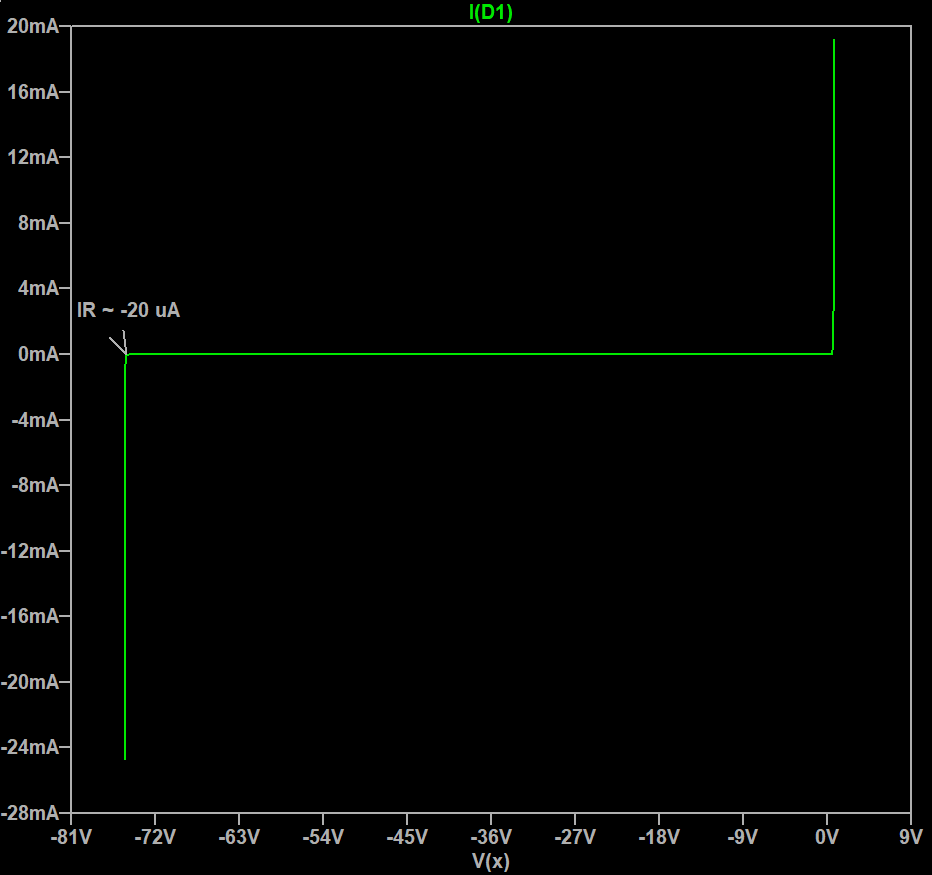
\includegraphics[width=\columnwidth]{img/gr1.1.png}
        \caption{Gráfica completa. Se encuentra marcada la corriente inversa de saturación.}
		\label{fig:gr1.1}
    \end{subfigure}
    \begin{subfigure}[t]{0.4\textwidth}
        \centering
        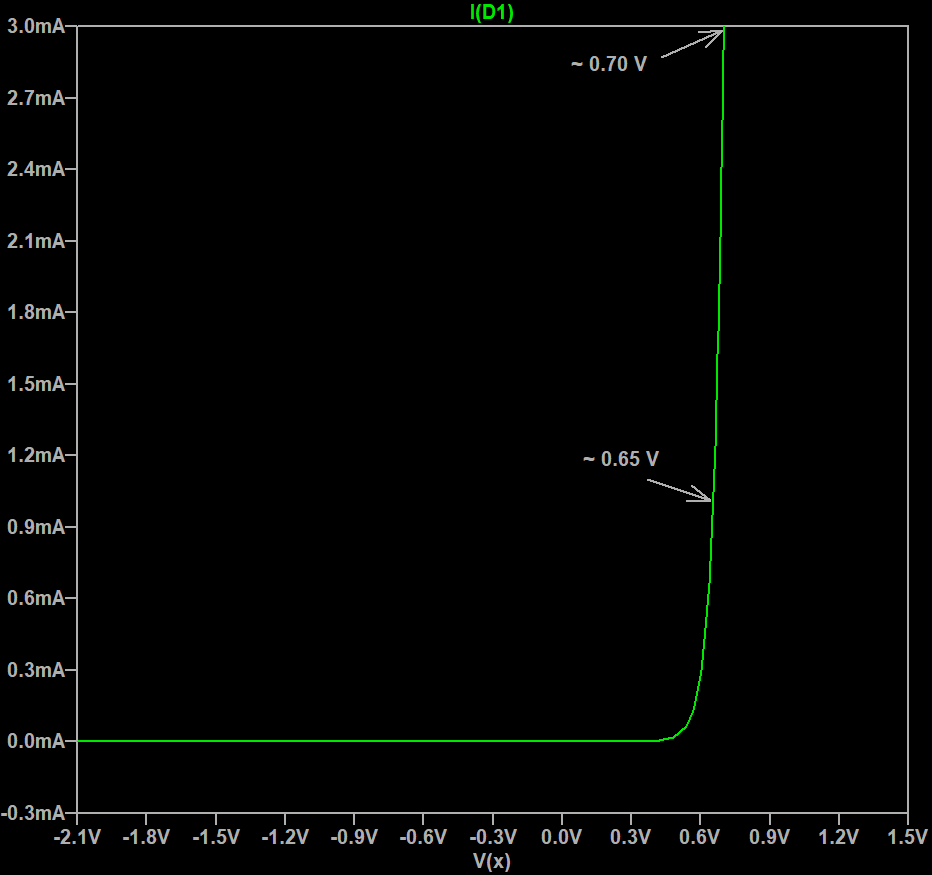
\includegraphics[width=\columnwidth]{img/gr1.1codo.png}
        \caption{Gráfica aumentada en la sección de inicio de conducción. Se encuentran indicados los voltajes para las distintas corrientes pedidas.}
		\label{fig:gr1.1codo}
    \end{subfigure}
    \caption{Gráfica característica I/V del diodo 1N4148.}
\end{figure}

\begin{wrapfigure}{r}{0.5\textwidth}
\centering
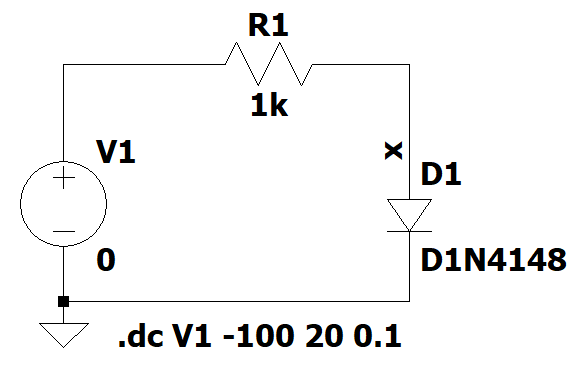
\includegraphics[width=0.95\columnwidth]{img/sch1.1.png}
\label{fig:sch1.1}
\caption{Esquema del circuito en LTspice}
\end{wrapfigure}

Se ha empleado el modelo del diodo 1N4148 que usa \textit{Qucs}, y se ha traducido con una directiva \code{.model} (ver Apéndice) en \textit{LTspice}.

Se puede observar que el diodo tiene una \textbf{tensión de ruptura} de aproximadamente $\boxed{-110\, V}$ para este modelo, como se puede observar en la \cref{fig:gr1.1}. Esta, por definición, se da cuando el diodo empieza a conducir en polarización inversa.

La \textbf{corriente inversa de saturación} es aquella que circula antes de la ruptura. En este diodo es entre el orden de nanoamperios y microamperios, y su valor máximo antes de la ruptura es aproximadamente $\boxed{-20 \,\mu A}$.

Tras hacer zoom en el inicio de la conducción (\cref{fig:gr1.1codo}), gráficamente observamos que la \textbf{tensión de codo} en \textbf{1 mA} es $\boxed{\approx 0.65\, V}$, y en \textbf{3 mA} es $\boxed{\approx 0.70\, V}$.

Se han hallado las \textbf{resistencias dinámicas} usando el operador diferencial (\code{D}) de LTspice. Primero se han guardado en variables las medidas de los voltajes $V_1$ cuando la intensidad es 1 y 3 mA (que coinciden precisamente con las medidas halladas gráficamente), y se han usado dichos valores en la función \code{.meas} para que coja las medidas $I_d$ y $V_d$ en esos punto del barrido Estas son las funciones empleadas:
\begin{codeblock}
	.meas dc V1a FIND V1 when I(D1)=1m
	.meas dc V3a FIND V1 when I(D1)=3m
	.meas dc rd1a FIND 1/(D(I(D1))/D(V(x))) AT=V1a
	.meas dc rd3a FIND 1/(D(I(D1))/D(V(x))) AT=V3a
\end{codeblock}

Los resultados son:
\begin{gather*}
	\boxed{r_d(1mA) = 42.93\, \Omega} \; ; \; \boxed{r_d(3mA) = 14.08\Omega}
\end{gather*}

\subsection{Tiempos de almacenamiento y transición}

\begin{figure}[h]
  \begin{floatrow}
	\ffigbox{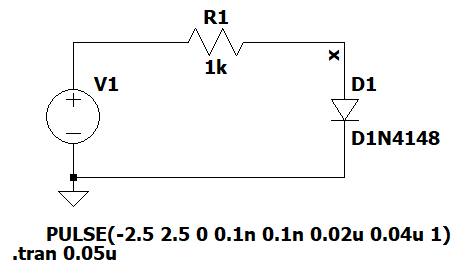
\includegraphics[width=0.7\columnwidth]{img/sch1.2.png}}
	{\caption{Esquema del circuito en LTspice.}
	\label{fig:sch1.2}}
	\ffigbox{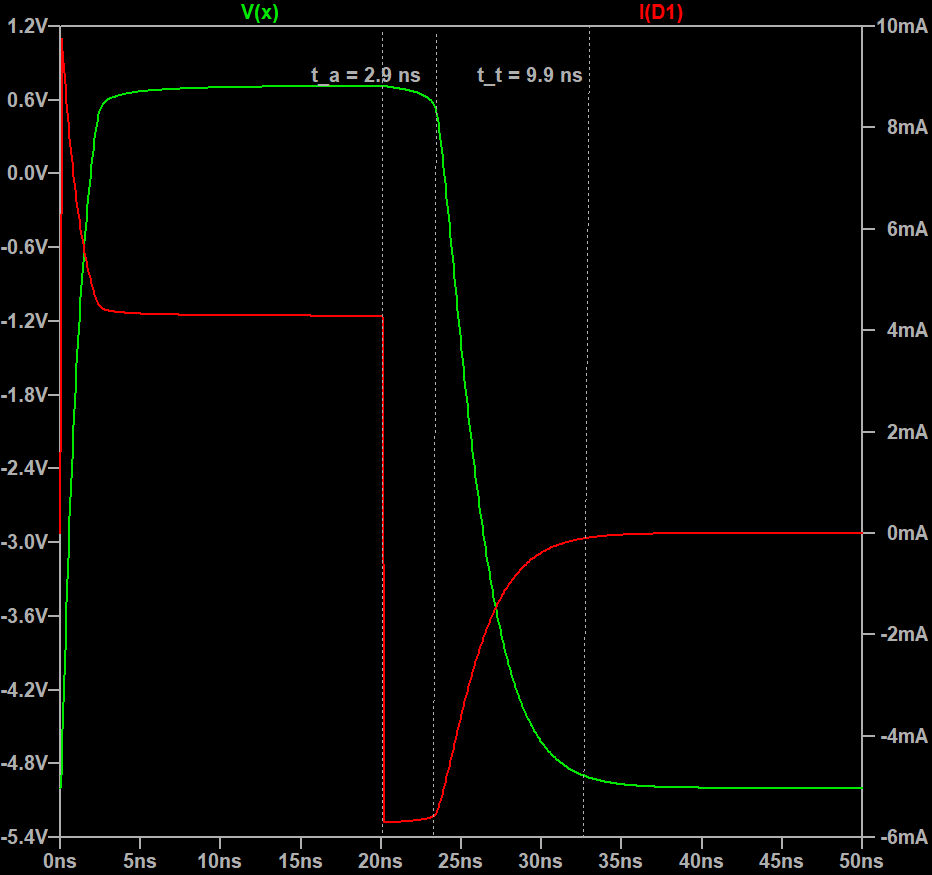
\includegraphics[width=0.7\columnwidth]{img/gr1.2.png}}
	{\caption{Evolución temporal del voltaje (verde) y la intensidad (roja) del diodo durante un ciclo. Se encuentran marcados los tiempos de almacenamiento (t\_a) y transición (t\_t).}
	\label{fig:gr1.2}}
  \end{floatrow}
\end{figure}

Gráficamente se ha representado un solo ciclo para poder ver los \textbf{tiempos} con claridad (\cref{fig:gr1.2}). Hemos hallado que el tiempo de almacenamiento es $\boxed{t_a=2.9\, ns}$, y el de transición $\boxed{t_t=9.9\, ns}$

La \textbf{capacidad media de difusión} se mide en un punto de polarización directa, mientras que la de \textbf{transición} se mide en polarización inversa. Se han obtenido usando \code{.meas} y aplicando la fórmula para los puntos necesarios $i(t)=C\frac{dv_d}{dt}$:
\begin{codeblock}
	.meas tran Cd FIND I(D1)/D(V(x)) AT=8n
	.meas tran Ct FIND I(D1)/D(V(x)) AT=35n
\end{codeblock}
	
Hallamos que:
\begin{gather*}
	\boxed{C_D = 8.98 \cdot 10^{-10}\, F}\; ; \; \boxed{C_T = 2.00 \cdot 10^{-12}\, F}
\end{gather*}

\section{Análisis del diodo Zener}

\subsection{Corriente inversa de saturación y voltaje Zener}

\begin{figure}[h]
  \begin{floatrow}
	\ffigbox{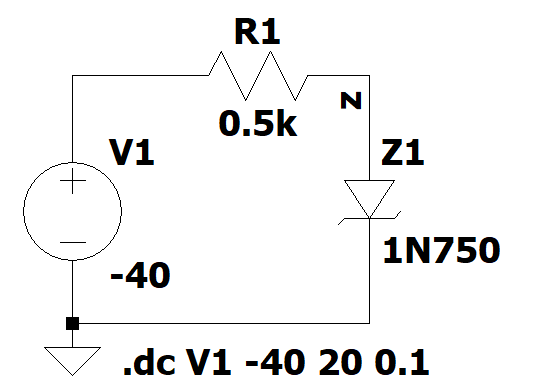
\includegraphics[width=0.7\columnwidth]{img/sch2.1.png}}
	{\caption{Esquema del circuito en LTspice.}
	\label{fig:sch2.1}}
	\ffigbox{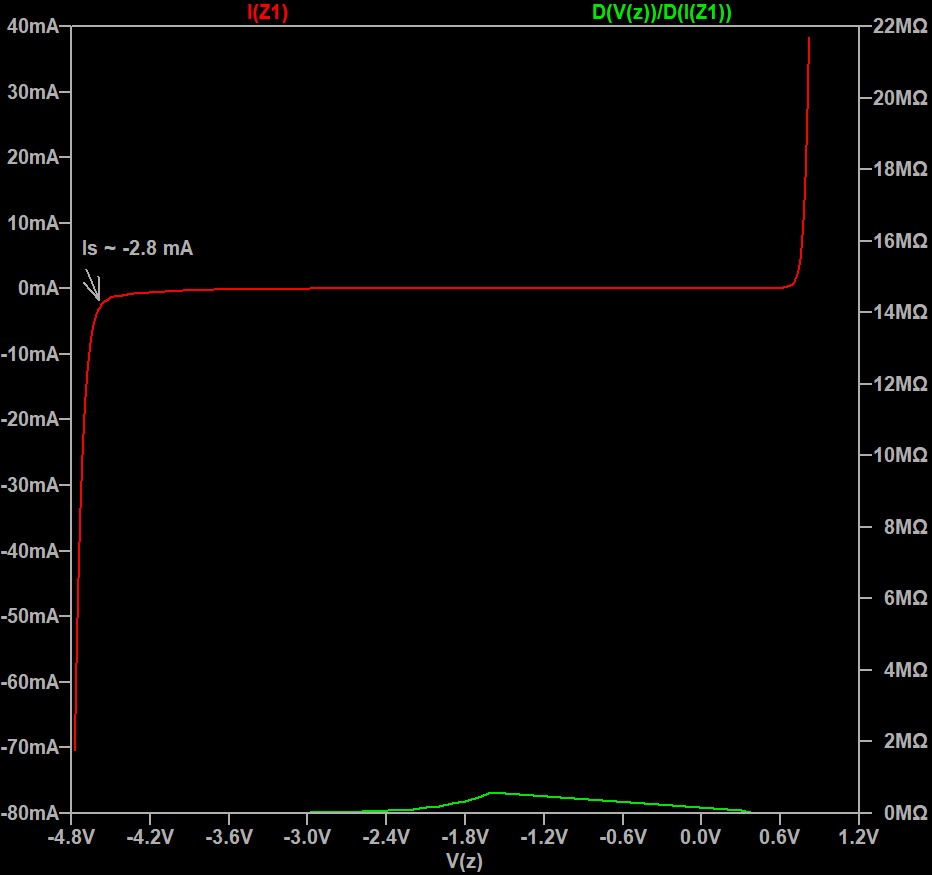
\includegraphics[width=0.7\columnwidth]{img/gr2.1.png}}
	{\caption{Gráfica de la corriente zener en el barrido de voltaje. Se incluye también los resultados de la impedancia, pero son \textbf{claramente erróneos}, como se indica en la sección 2.2.}
	\label{fig:gr2.1}}
  \end{floatrow}
\end{figure}

\textit{\textbf{Nota:} Ha habido que subir el voltaje final a 20 V ya que, en el cálculo de los voltajes zener para corrientes de saturación, quedaban fuera de los límites los de 20 y 30 mA.}

Tras realizar el barrido de voltaje (\cref{fig:gr2.1}), hallamos gráficamente que la \textbf{corriente inversa de saturación máxima} es $\boxed{I_s = -2.8\, mA}$

Se han calculado los \textbf{voltajes zener} para las distintas intensidades con la función \code{.meas}:
\begin{codeblock}
	.meas dc Vz10 FIND V(z) WHEN I(Z1)=10m
	.meas dc Vz20 FIND V(z) WHEN I(Z1)=20m
	.meas dc Vz30 FIND V(z) WHEN I(Z1)=30m
\end{codeblock}

Obteniendo:
\begin{gather*}
	\boxed{V_z(10mA) = 0.78\, V}\; ; \; \boxed{V_z(20mA) = 0.80\, V} \; ; \; \boxed{V_z(30mA) = 0.81\, V}
\end{gather*}

\subsection{Impedancia Zener}

Se ha añadido la ecuación de la \textbf{impedancia} insertando la traza \code{1/(D(I(Z1))/D(V(z)))} en la \cref{fig:gr2.1}, pero devuelve valores inesperados. Es posible que sea un error del software pero no he sido capaz de resolverlo. 

Esperaríamos que $r_z$ empezase muy alto en polarización inveresa, caería bruscamente en la tensión de zener y tras la ruptura se estabilizaría en unos pocos ohmios. Esto claramente no coincide con lo obtenido, que además se encuentra en el orden de megaohmios.

\section{Rectificación}

\subsection{Rectificador de media onda}

\begin{figure}[th!]
	\centering
	\begin{subfigure}[t]{0.4\textwidth}
		\centering
		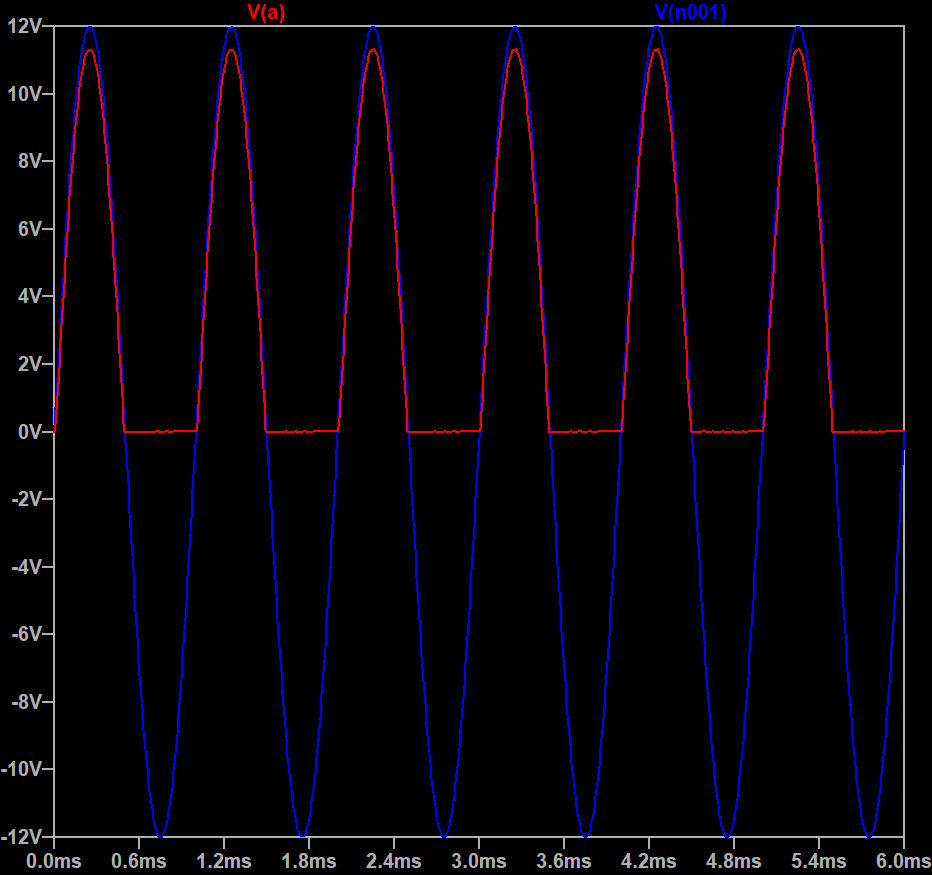
\includegraphics[width=\columnwidth]{img/gr3.1}
		\caption{}
		\label{fig:gr3.1}
	\end{subfigure}
	\begin{subfigure}[t]{0.4\textwidth}
		\centering
		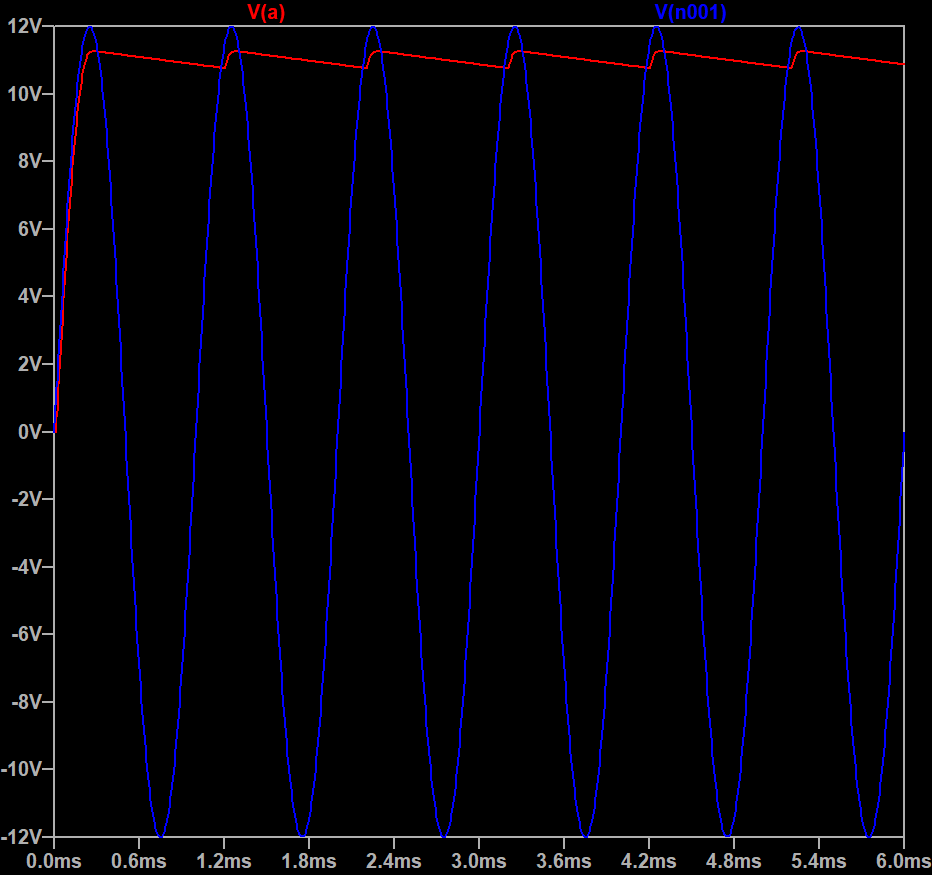
\includegraphics[width=\columnwidth]{img/gr3.1riz.png}
		\caption{}
		\label{fig:gr3.1riz}
	\end{subfigure}
	\caption{}
\end{figure}
\begin{wrapfigure}[10]{r}{0.45\textwidth}
\vspace{-1.7cm}
\centering
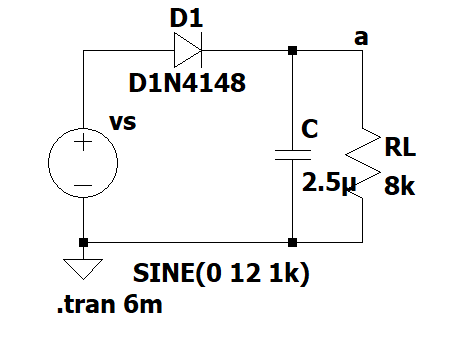
\includegraphics[width=0.95\columnwidth]{img/sch3.1.png}
\label{fig:sch3.1}
\caption{Esquema del circuito en LTspice (para la primera parte del ejercicio se ha desconectado el condensador).}
\end{wrapfigure}

Para el caso del circuito \textbf{sin condensador}, observamos que el diodo filtra la parte negativa de la señal y sólo queda la positiva (\cref{fig:gr3.1}), quedando 0 V donde habían valores negativos y perdiendo la mitad de la señal. La señal resultante tiene una amplitud (sólo positiva) ligeramente menor que 12 V por la caída de tensión del propio diodo, ya que no es ideal.

Para hallar el valor de la \textbf{capacidad del condensador} con el que tendremos un $V_{rizado}=0.05V_{max}$, sustituimos dicha relación en la fórmula proporcionada:
\begin{gather*}
	V_{rizado}=\frac{V_{max}}{fR_L C} \Rightarrow C = \frac{1}{0.05fR_L} = \boxed{2.5\, \mu F}
\end{gather*} 

En la \cref{fig:gr3.1riz} observamos que para el voltaje de salida tras añadir el condensador, sus valores máximo y mínimo son $Vr_{max}= 11.27\, V\; \text{y} \; Vr_{min} =10.76\, V$. Podemos calcular su \textbf{voltaje de rizado} simplemente restándolos. Observamos que coincide aproximadamente con el rizado pedido ($5\%$):
\begin{gather}
	V_{rizado} = Vr_{max} - Vr_{min} = \boxed{0.51\, V}\, \approx 0.05V_{max}
\end{gather}

El \textbf{valor medio de la tensión de salida} será simplemente $\frac{Vr_{max}+Vr_{min}}{2} = \boxed{11.02\, V}$. Se puede deducir una expresión para diodos ideales, que sirve como aproximación para diodos que no disipen mucho voltaje (sería apto para el diodo usado), en los que $Vr_{max} \approxeq V_{max}$, siendo $V_{max}$ la amplitud del voltaje de entrada:
\begin{gather*}
	V_{med}=\frac{V_{max}+(V_{max}-V_{riz})}{2} \Rightarrow \boxed{V_{med} \approxeq V_{max}-\frac{V_{riz}}{2}}
\end{gather*}

\subsection{Rectificador de onda completa}

.\begin{figure}[th!]
	\centering
	\begin{subfigure}[t]{0.4\textwidth}
		\centering
		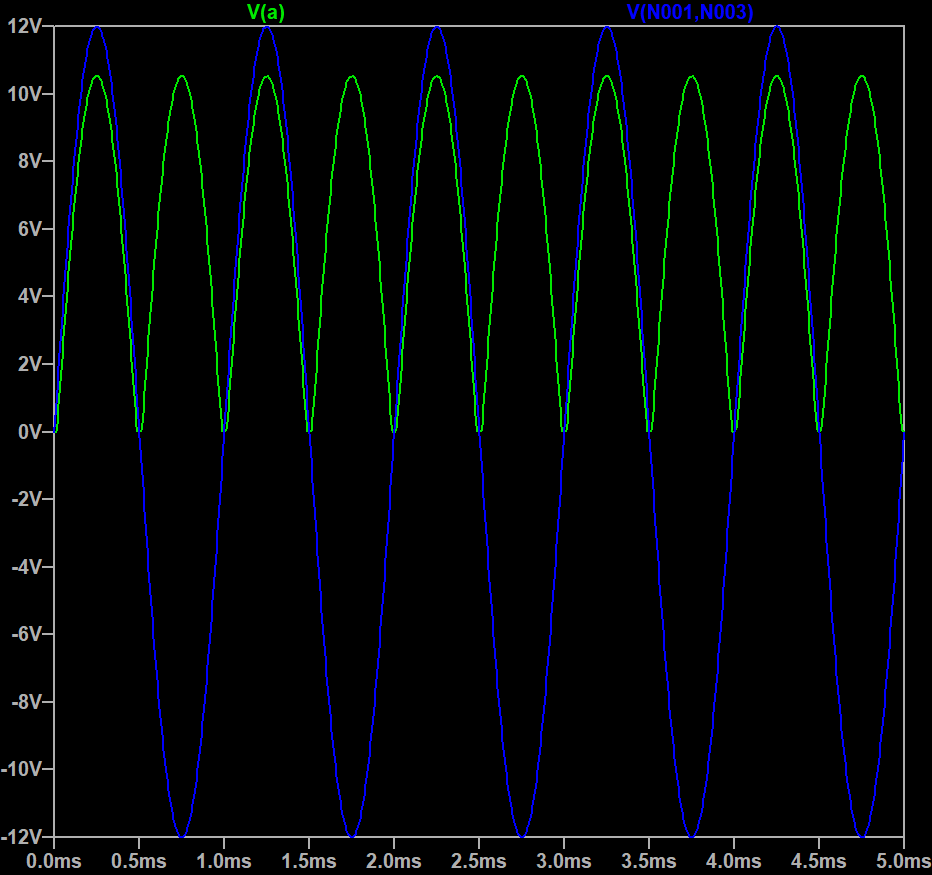
\includegraphics[width=\columnwidth]{img/gr3.2.png}
		\caption{Señales obtenidas sin el condensador.}
		\label{fig:gr3.2}
	\end{subfigure}
	\begin{subfigure}[t]{0.4\textwidth}
		\centering
		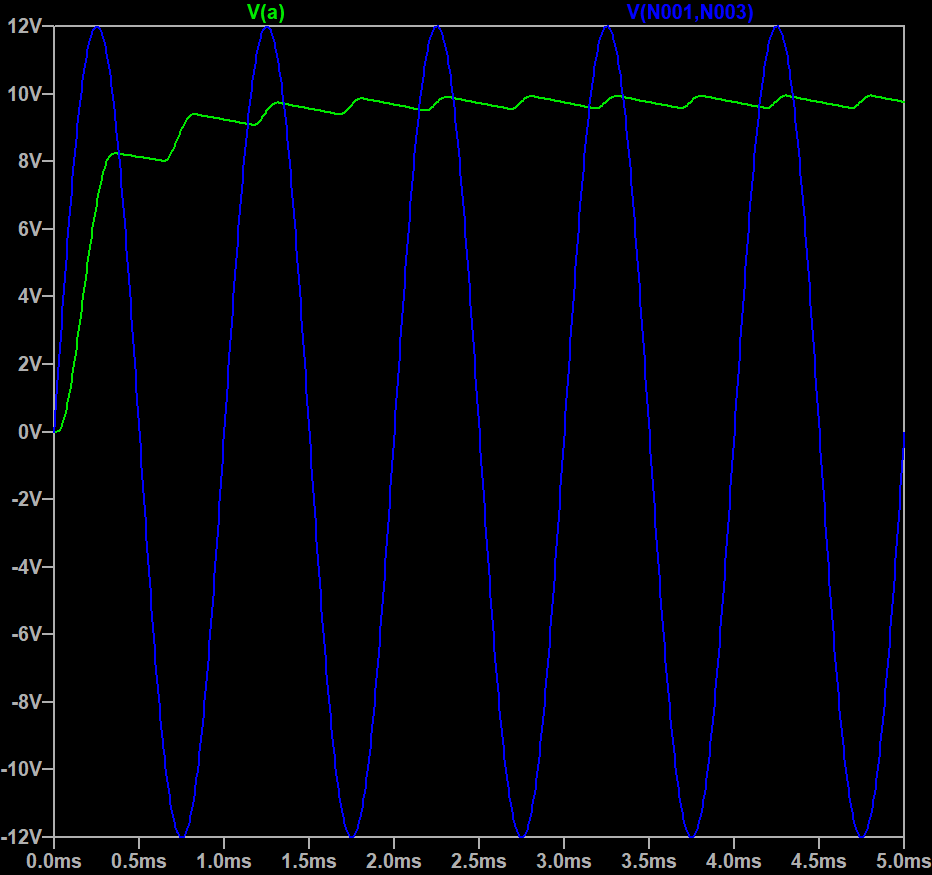
\includegraphics[width=\columnwidth]{img/gr3.2riz.png}
		\caption{Señale obtenidas tras añadir un condensador de 1.25 $\mu$F.}
		\label{fig:gr3.2riz}
	\end{subfigure}
	\caption{Gráficas ilustrando 5 ciclos de la señal generada por la fuente (azul) y la rectificada (verde).}
\end{figure}

\begin{wrapfigure}{r}{0.5\textwidth}
\centering
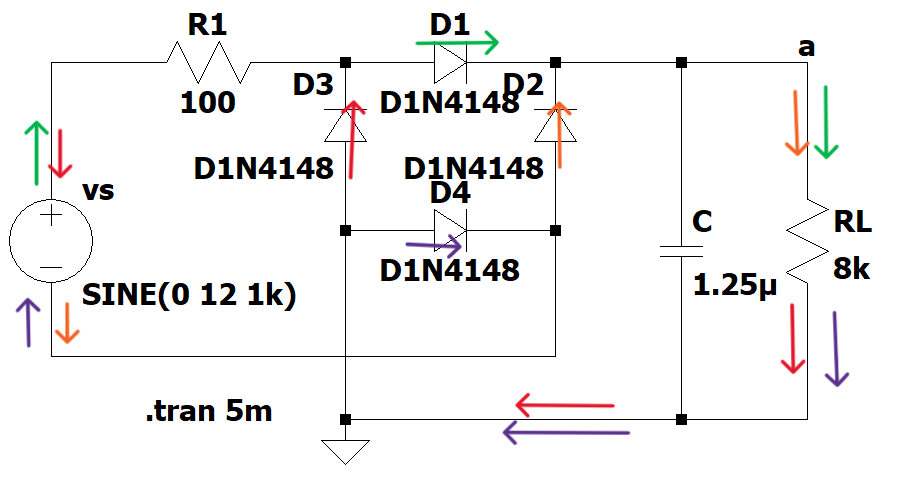
\includegraphics[width=0.95\columnwidth]{img/sch3.2.png}
\label{fig:sch3.2}
\caption{Esquema del circuito en LTspice. Las flechas verdes y moradas corresponden con la entrada y salida del ciclo positivo respectivamente, y las naranjas y rojas a la entrada y salida del ciclo negativo.}
\end{wrapfigure}

Este circuito permite convertir el semiciclo negativo en voltaje positivo, ``dándole la vuelta'' a la parte negativa de la onda, sin perderla, como se puede observar en la \cref{fig:gr3.2}. El voltaje de salida es algo menor que el generado, más notablemente que en el ejercicio anterior, debido a que en este caso hay cuatro diodos no ideales con una caída de tensión cada uno (dos para cada ciclo). Llamaremos al valor máximo de éste $V'_{max}$ para futura referencia.

El sentido de la corriente no cambia con la polaridad gracias a los diodos, que la dirigen hacia el borne correspondiente dependiendo del ciclo en el que esté. El \textbf{camino recorrido en cada ciclo} se encuentra ilustrado en la \cref{fig:sch3.2}.

Análogo al ejercicio anterior (pero con la fórmula de onda completa), para hallar el valor de la \textbf{capacidad del condensador} para el rizado deseado ($5\%$) hacemos:
\begin{gather*}
	V_{riz} = \frac{V_{max}}{2fR_L C} \Rightarrow C= \frac{1}{0.05\cdot 2fR_L} = \boxed{1.25\, \mu F}
\end{gather*}

\textbf{Tras añadir el condensador}, observamos en la \cref{fig:gr3.2riz} que durante los dos primeros ciclos aún no se ha cargado del todo. A partir de ahí se estabiliza, por lo que podemos hallar el rizado gráficamente y comprobar el resultado con el mismo método empleado anteriormente:
\begin{gather*}
	V_{riz} = Vr_{max}-Vr_{min} = 9.94 - 9.58 = \boxed{0.36\, V} \, \approx 0.05V'_{max} \, < 0.05 V_{max}
\end{gather*}

\section{Fuente de alimentación contínua}

\subsection{Reducción del rizado}

\begin{figure}[th!]
	\centering
	\begin{subfigure}[t]{0.4\textwidth}
		\centering
		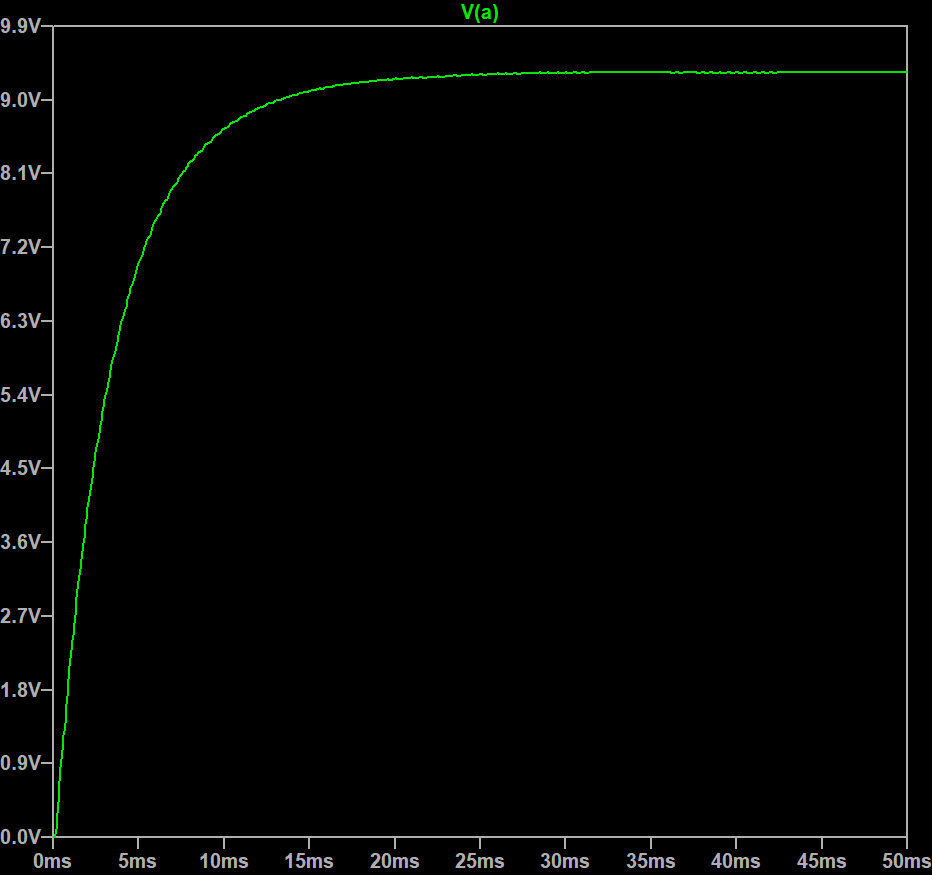
\includegraphics[width=\columnwidth]{img/gr4.1.png}
		\caption{Voltaje de salida con la carga de 8k ohmios.}
		\label{fig:gr4.1}
	\end{subfigure}
	\begin{subfigure}[t]{0.4\textwidth}
		\centering
		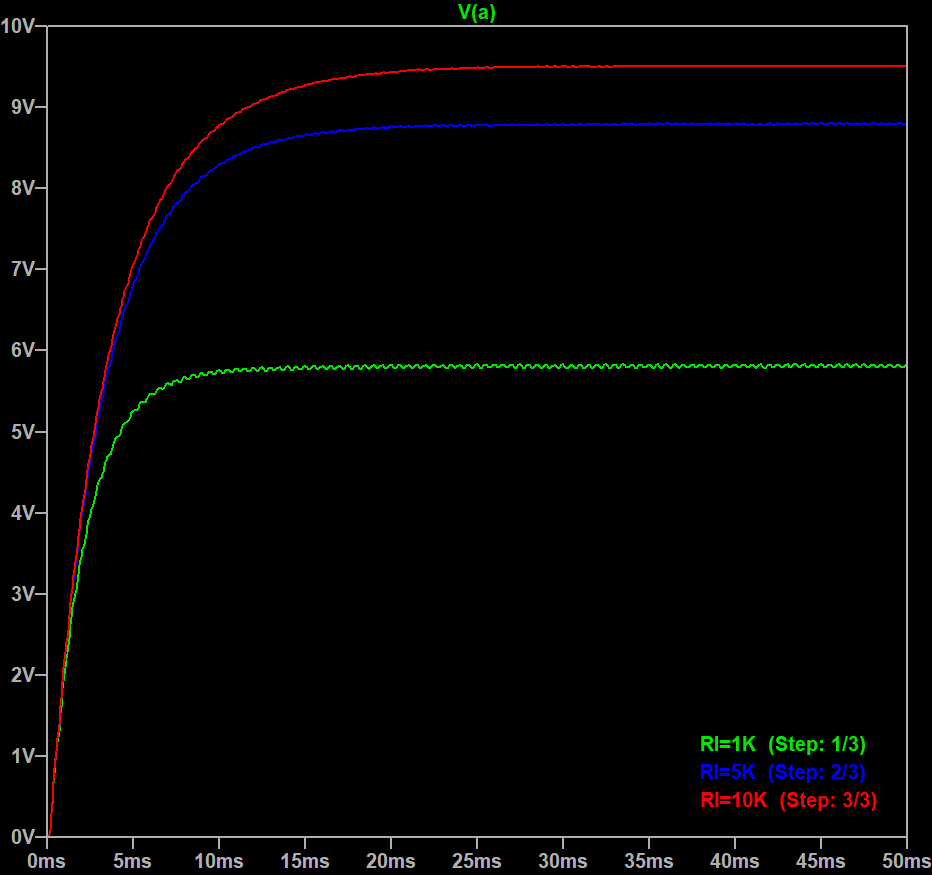
\includegraphics[width=\columnwidth]{img/gr4.1res.png}
		\caption{Voltaje de salida para 1k, 5k y 10k ohmios.}
		\label{fig:gr4.1res}
	\end{subfigure}
	\caption{Gráficas de la evolución del voltaje con el tiempo.}
\end{figure}

\begin{wrapfigure}{r}{0.5\textwidth}
\centering
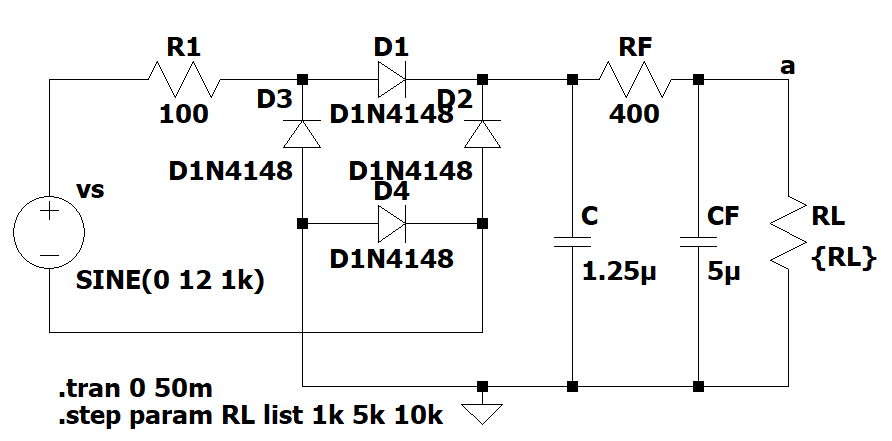
\includegraphics[width=0.95\columnwidth]{img/sch4.1.png}
\label{fig:sch4.1}
\caption{Esquema del circuito en LTspice con los valores de los componentes escogidos y la resistencia $R_L$ como variable que será sustituida por la función \code{.step}.}
\end{wrapfigure}

Tras probar varias combinaciones, se ha elegido una resistencia de 400 ohm, relativamente pequeña comparada con la carga, para que no haya mucha caída de tensión, y se ha añadido un condensador con una capacidad de 5 uF que, aunque provoca que el voltaje de salida tarde 20ms en estabilizarse del todo una vez encendido, nos da una señal bastante limpia de aproximadamente 9.33 $\pm$ 0.01 V, como se aprecia en la \cref{fig:gr4.1}.

Para hacer el \textbf{análisis paramétrico}, se ha sustituido el valor de la resistencia de carga por una variable \code{RL} y se ha usado \code{.step} para graficar las tres curvas a la vez. Observamos en la \cref{fig:gr4.1res} que el voltaje es mayor cuanto mayor sea la resistencia, como era de esperar según la ley de Ohm. También se aprecia que la traza de la resistencia de 1k es notablemente más ``ondulada'' que las resistencias mayores, y esto puede ser debido a que, como causa que el voltaje de salida sea menor, el condensador no se carga del todo y no es capaz de compensar la señal con la misma eficiencia.

\subsection{Regulador Zener}

\begin{figure}[h]
  \begin{floatrow}
	\ffigbox{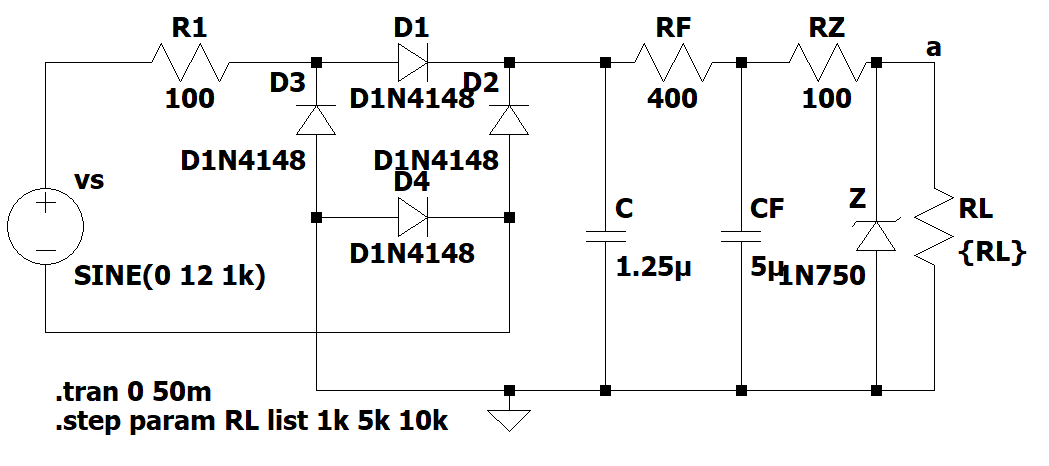
\includegraphics[width=0.7\columnwidth]{img/sch4.2.png}}
	{\caption{Esquema del circuito en LTspice.}
	\label{fig:sch4.2}}
	\ffigbox{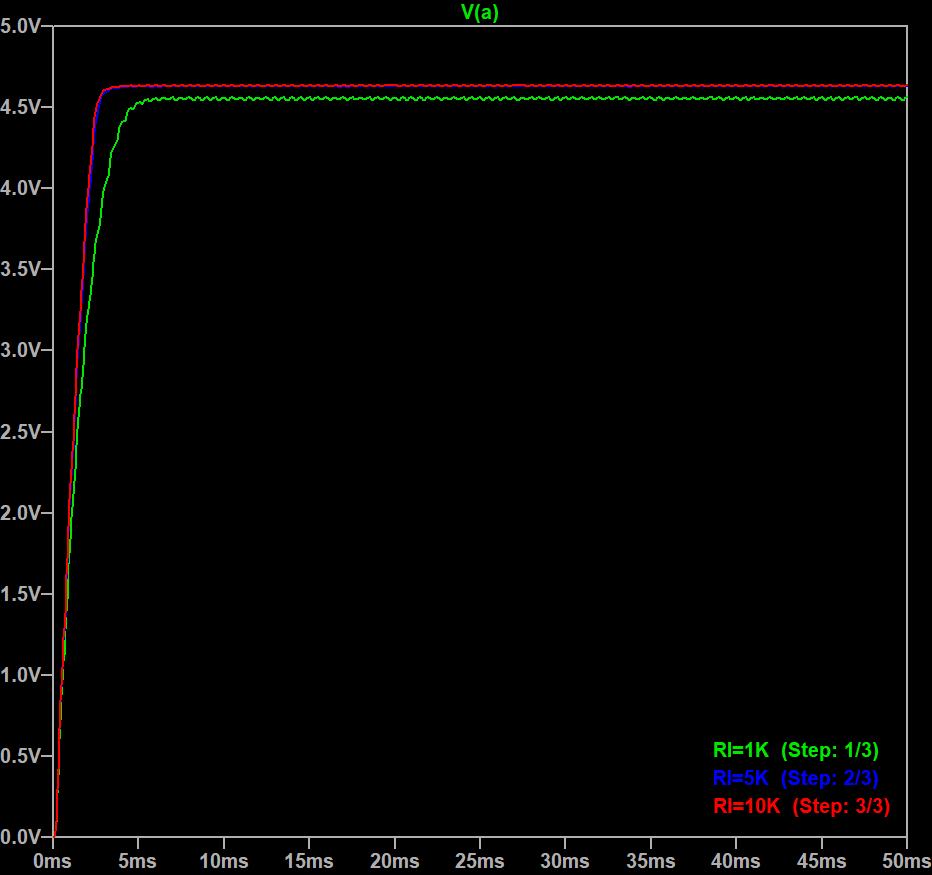
\includegraphics[width=0.7\columnwidth]{img/gr4.2.png}}
	{\caption{Gráfica V/t para cada valor de resistencia estudiado.}
	\label{fig:gr4.2}}
  \end{floatrow}
\end{figure}

Al añadir el regulador Zener, se ha observado que la amplitud de la onda de la resistencia menor (1k) ha \textbf{bajado} de 0.03 a 0.01 V. Es una cantidad pequeña, pero a otras escalas o con diodos diferentes podría tener más influencia. También \textbf{reduce el voltaje} acorde al que el regulador Zener dicta, que en este caso parece tener un máximo alrededor de 4.64 V, ya que tanto la resistencia de 5k como la de 10k producen este mismo voltaje de salida, como se puede observar en la \cref{fig:gr4.1res}.

%_________________________________________

%\nocite{*}
%\printbibliography

\appendix
\textbf{APÉNDICE} \label{app:appendix}

$\bullet$\textbf{Modelo de Qucs adaptado a LTSpice del diodo 1N4148:} 
.model D1N4148 D(IS=222p N=1.65 CJO=4p M=0.333 VJ=0.7 FC=0.5 RS=68.6m TT=5.76n BV=75 IBV=1u XTI=3 EG=1.11)

\clearpage

\vspace{2cm}
\begin{center}
\setlength{\fboxsep}{0.5cm}
\shadowbox{\begin{minipage}{10.5cm}
\textbf{Declaración de Autoría}\\

El alumno
Álvaro Jerónimo Sánchez
, con DNI número 
09847051S
, declara que es el autor único e individual de este trabajo.\\

\vspace{3cm}
Fdo:

\end{minipage}}
\end{center}

\end{document}